\documentclass{beamer}
\usepackage[english,russian]{babel}
\usepackage[utf8]{inputenc}
\usepackage{amsmath}
\usepackage{hyperref}
\usetheme{Warsaw}
\usepackage{listings}
\usepackage{xcolor}
\usepackage{tikz}
\usetikzlibrary{graphs}
\usepackage{algpseudocode}

\lstset{
    frame=tb,
    tabsize=4,
    showstringspaces=false,
    numbers=left,
    commentstyle=\color{green},
    keywordstyle=\color{blue},
    stringstyle=\color{red},
    emph={baz},
    emphstyle=\textbf
}

\begin{document}

\title{Задачи разрешимости логических формул и приложения\newline Лекция 8. Логика указателей}
\author{Роман Холин}
\institute{Московский государственный университет}
\date{Москва, 2022}

\begin{frame}
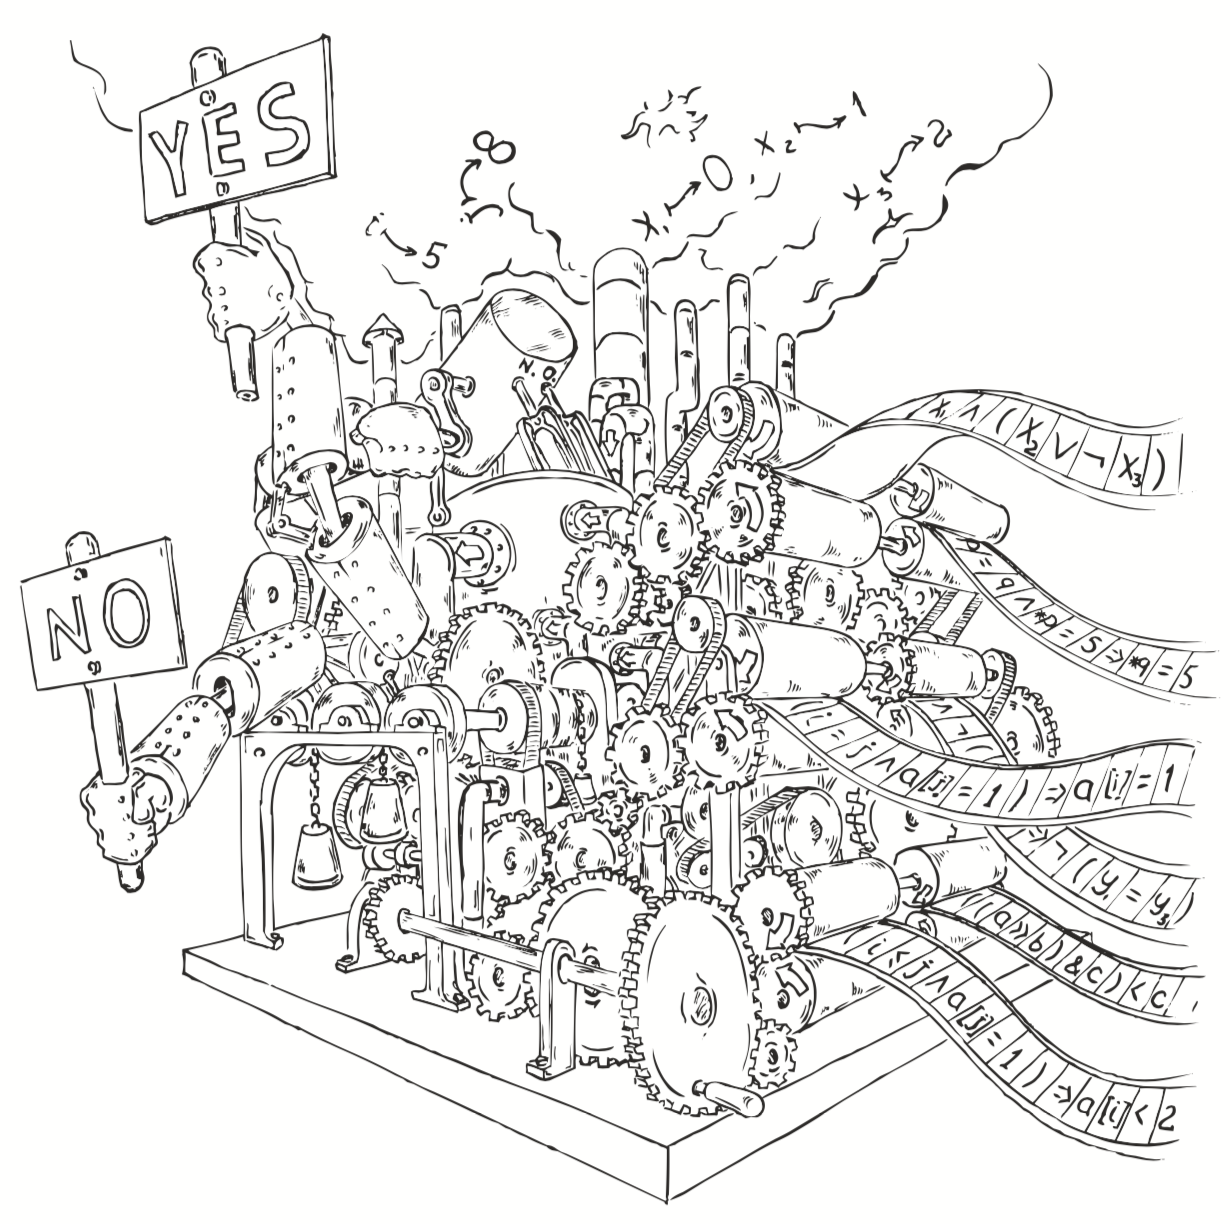
\includegraphics[scale=0.5]{../decision-procedure.png}
\end{frame}

\frame{\titlepage}

\begin{frame}{Модель памяти}
\begin{itemize}
\item $V$ - множество переменных
\item $A$ - множество адресов ($\{0, \dots, n-1\}$)
\item $D$ - множество слов
\item Оценка памяти $M$ - отображение из  $A$ в $D$
\item $\sigma(v)$ - размер переменной (в словах)
\item $L$ - отображение из $V$ в $A$ - расположение памяти
\end{itemize}
\end{frame}

\begin{frame}{Пример}
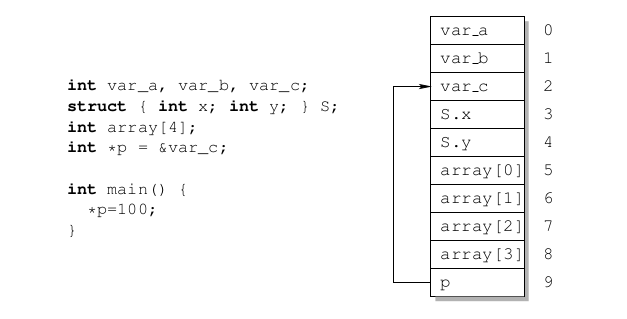
\includegraphics[scale=0.5]{layout.png}
\end{frame}

\begin{frame}{Пример}
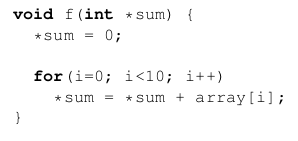
\includegraphics[scale=0.5]{ex1.png}
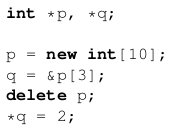
\includegraphics[scale=0.5]{ex2.png}
\end{frame}

\begin{frame}{Синтаксис}
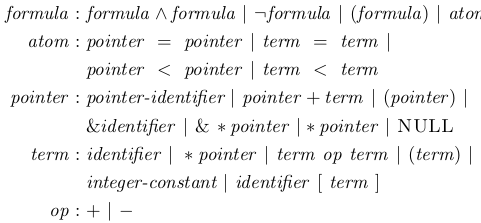
\includegraphics[scale=0.5]{syntax.png}
\end{frame}

\begin{frame}{Пример}
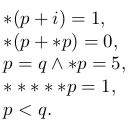
\includegraphics[scale=0.5]{perm.png}
\end{frame}

\begin{frame}{Пример}
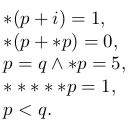
\includegraphics[scale=0.5]{perm.png}
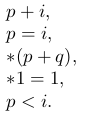
\includegraphics[scale=0.5]{not_perm.png}
\end{frame}

\begin{frame}{Семантика}
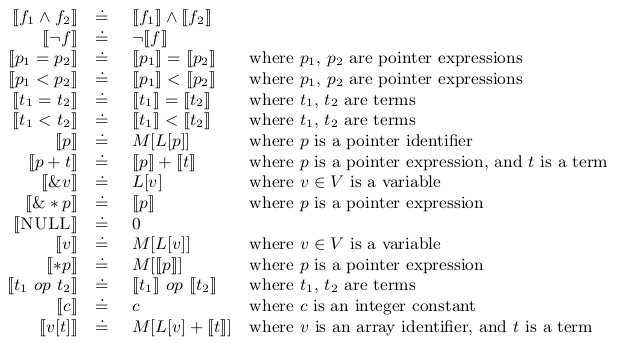
\includegraphics[scale=0.5]{semantics.png}
\end{frame}

\begin{frame}{Пример}
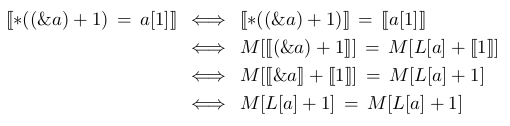
\includegraphics[scale=0.5]{semantics_ex.png}
\end{frame}

\begin{frame}{Аксиомы}
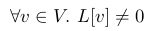
\includegraphics[scale=0.5]{axiom1.png}\newline
\end{frame}

\begin{frame}{Аксиомы}
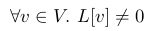
\includegraphics[scale=0.5]{axiom1.png}\newline
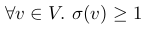
\includegraphics[scale=0.5]{axiom2.png}\newline
\end{frame}

\begin{frame}{Аксиомы}
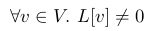
\includegraphics[scale=0.5]{axiom1.png}\newline
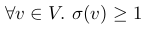
\includegraphics[scale=0.5]{axiom2.png}\newline
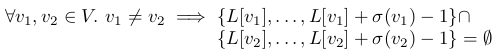
\includegraphics[scale=0.5]{axiom3.png}
\end{frame}

\begin{frame}{Структуры}
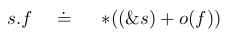
\includegraphics[scale=0.5]{struct1.png}\newline
\end{frame}

\begin{frame}{Структуры}
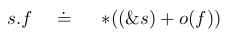
\includegraphics[scale=0.5]{struct1.png}\newline
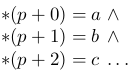
\includegraphics[scale=0.5]{struct2.png}\newline
\end{frame}

\begin{frame}{Разрешающая процедура}
\begin{itemize}
\item Логика указателей сводится к догике массивов
\item Благодаря семантической трансляции формула из логики указателей транслируется в формулу из логики массивов с операцией
чтения; логика индексов - линейная арифметика либо битовые вектора
\item Единственная проблема - кванторы
\end{itemize}
\end{frame}

\begin{frame}{Пример}
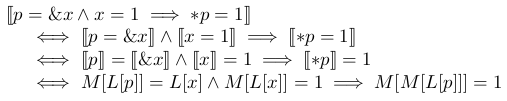
\includegraphics[scale=0.5]{ex_good.png}\newline
\end{frame}

\begin{frame}{Пример}
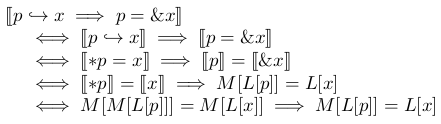
\includegraphics[scale=0.5]{ex_bad1.png}\newline
\end{frame}

\begin{frame}{Пример}
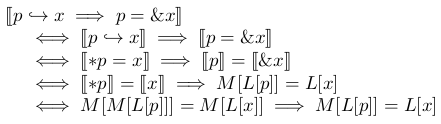
\includegraphics[scale=0.5]{ex_bad1.png}\newline
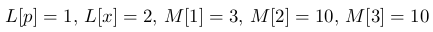
\includegraphics[scale=0.5]{ex_bad2.png}\newline
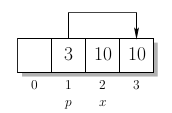
\includegraphics[scale=0.5]{ex_bad3.png}\newline
\end{frame}

\begin{frame}{Оптимизация: применение аксиомы модели памяти}
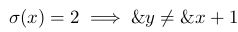
\includegraphics[scale=0.5]{meory1.png}\newline
\end{frame}

\begin{frame}{Оптимизация: применение аксиомы модели памяти}
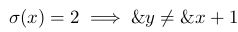
\includegraphics[scale=0.5]{meory1.png}\newline
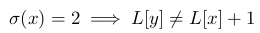
\includegraphics[scale=0.5]{meory2.png}\newline
\end{frame}

\begin{frame}{Оптимизация: применение аксиомы модели памяти}
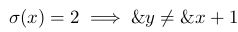
\includegraphics[scale=0.5]{meory1.png}\newline
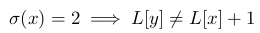
\includegraphics[scale=0.5]{meory2.png}\newline
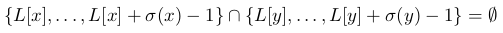
\includegraphics[scale=0.5]{meory3.png}\newline
\end{frame}

\begin{frame}{Оптимизация: применение аксиомы модели памяти}
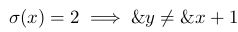
\includegraphics[scale=0.5]{meory1.png}\newline
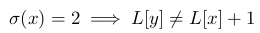
\includegraphics[scale=0.5]{meory2.png}\newline
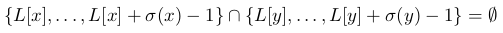
\includegraphics[scale=0.5]{meory3.png}\newline
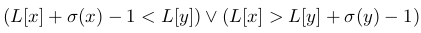
\includegraphics[scale=0.5]{meory4.png}\newline
\end{frame}

\begin{frame}{Оптимизация: применение аксиомы модели памяти}
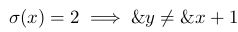
\includegraphics[scale=0.5]{meory1.png}\newline
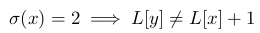
\includegraphics[scale=0.5]{meory2.png}\newline
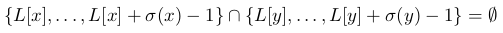
\includegraphics[scale=0.5]{meory3.png}\newline
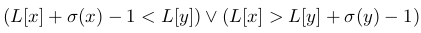
\includegraphics[scale=0.5]{meory4.png}\newline
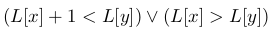
\includegraphics[scale=0.5]{meory5.png}\newline
\end{frame}

\begin{frame}{Оптимизация: чистые переменные}
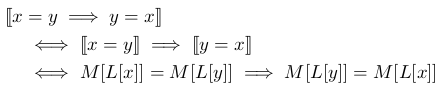
\includegraphics[scale=0.5]{ex_pure.png}\newline
\end{frame}

\begin{frame}{Оптимизация: чистые переменные}
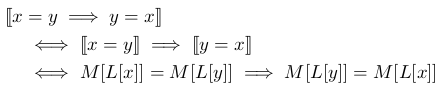
\includegraphics[scale=0.5]{ex_pure.png}\newline
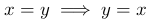
\includegraphics[scale=0.5]{ex_pure2.png}\newline
\end{frame}

\begin{frame}{Оптимизация: чистые переменные}
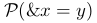
\includegraphics[scale=0.5]{pure1.png}\newline
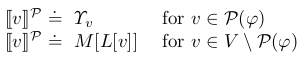
\includegraphics[scale=0.5]{pure2.png}\newline
\end{frame}

\begin{frame}{Оптимизация: чистые переменные}
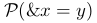
\includegraphics[scale=0.5]{pure1.png}\newline
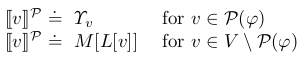
\includegraphics[scale=0.5]{pure2.png}\newline
Теорема:\newline
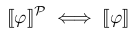
\includegraphics[scale=0.5]{theorem.png}\newline
\end{frame}

\begin{frame}{Оптимизация: чистые переменные}
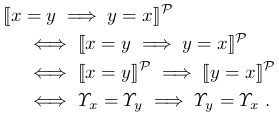
\includegraphics[scale=0.5]{ex_pure3.png}\newline
\end{frame}

\begin{frame}
\end{frame}

\begin{frame}
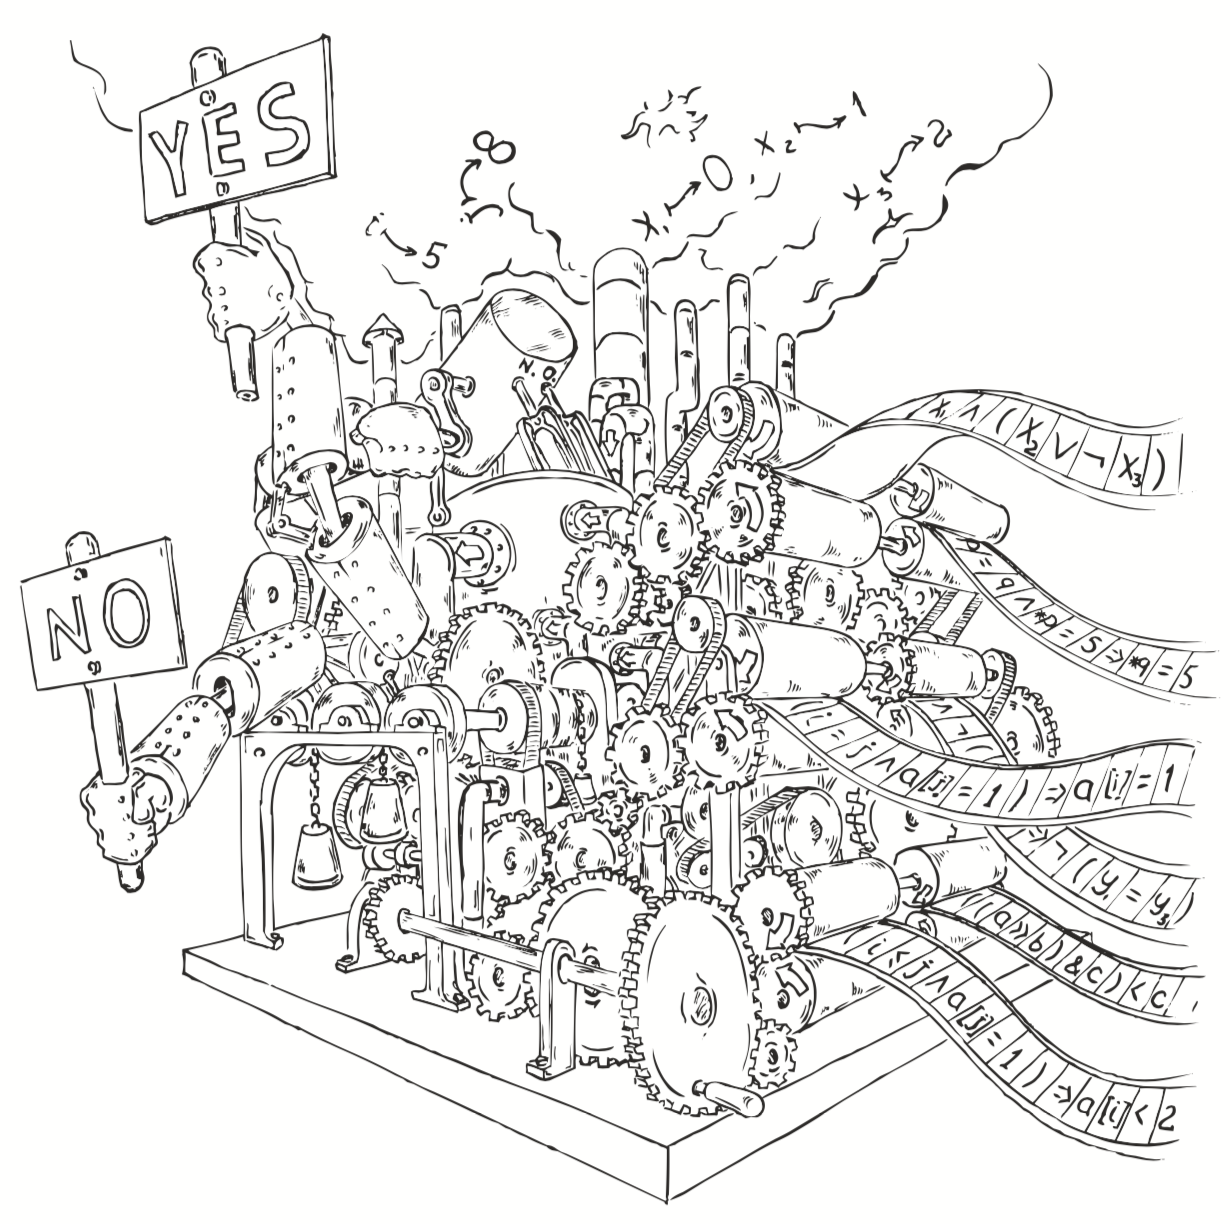
\includegraphics[scale=0.5]{../decision-procedure.png}
\end{frame}

\end{document}
